% =====================================================================
%  final-presentation.tex
%  EIL summer final presentation — Metropolis beamer theme
%  Slides are headline/visual only — full talking points in speaker-notes.md
%  Compile with: pdflatex final-presentation.tex
% =====================================================================
\documentclass[10pt,aspectratio=169]{beamer}
\usetheme{metropolis}

% ---- Brand colors (matches formats/research-highlight/_style.tex) ---
\definecolor{eilmaroon}{HTML}{641111}
\definecolor{eilink}{HTML}{1D2620}
\definecolor{eilpaper}{HTML}{FAF8F1}
\definecolor{eilwarmrule}{HTML}{D8D2C2}

\setbeamercolor{palette primary}{bg=eilmaroon,fg=white}
\setbeamercolor{frametitle}{bg=eilmaroon,fg=white}
\setbeamercolor{title separator}{fg=eilmaroon}
\setbeamercolor{progress bar}{fg=eilmaroon,bg=eilpaper}
\setbeamercolor{alerted text}{fg=eilmaroon}
\setbeamercolor{normal text}{fg=eilink}

% ---- Fonts (Source Sans, matching the rest of the output library) ---
\usepackage[T1]{fontenc}
\usepackage[default]{sourcesanspro}

\usepackage{graphicx}
\usepackage{booktabs}
\usepackage{array}
\usepackage{tcolorbox}
\tcbuselibrary{skins}

% ---- Helper for the option-card row ----------------------------------
\newcommand{\optioncard}[2]{%
  \begin{minipage}[t]{0.23\textwidth}
    \centering
    \includegraphics[width=\linewidth]{#1}\\[2pt]
    {\tiny #2}
  \end{minipage}}

\title{The EIL Output Library}
\subtitle{Translating Research for Public Audiences}
\author{Winn Philpott \\ Environmental Inequality Lab}
\date{Summer 2026}
\titlegraphic{\includegraphics[width=1.8cm]{../../formats/logos/eil-logo-maroon.png}}

\begin{document}

\maketitle

% ---------------------------------------------------------------------
\begin{frame}{The Project}
  \begin{center}
    \Large
    UVA and Batten's research rarely reaches audiences beyond academia.\\[14pt]
    \textbf{Goal:} centralized, replicable, shareable
  \end{center}
\end{frame}

% ---------------------------------------------------------------------
\begin{frame}{My Work}
  \begin{center}
    \large Learning by doing.

    \vspace{10pt}
    \Large
    Paper $\rightarrow$ Write $\rightarrow$ Iterate w/ PIs $\rightarrow$ Outputs

    \vspace{10pt}
    \normalsize Different goals $\rightarrow$ different formats
  \end{center}
\end{frame}

% ---------------------------------------------------------------------
\begin{frame}{Infrastructure I Built}
  \begin{center}
  \begin{tcolorbox}[colback=eilpaper,colframe=eilwarmrule,arc=3pt,boxrule=0.6pt,
                     width=0.92\textwidth,left=10pt,right=10pt,top=6pt,bottom=6pt]
    \ttfamily\footnotesize
    \textcolor{eilmaroon}{\textbf{papers/}}\\
    \hspace{1em}2026-epa-compliance-workshops/\\
    \hspace{2em}data-viz/ ~ research-highlight/ ~ press-release/ ~ blog/ ~ social/\\
    \hspace{1em}2025-early-life-pollution/ ~ WP-coal-worker-transitions/ ~ (+3 more)\\[4pt]
    \textcolor{eilmaroon}{\textbf{formats/}}\\
    \hspace{1em}research-highlight/ ~ press-release/ ~ social/ ~ data-viz/ ~ blog/ ~ logos/\\[4pt]
    \textcolor{eilmaroon}{\textbf{style-guides/}}\\
    \hspace{1em}research-highlight/ ~ press-release/ ~ social/ ~ data-viz/ ~ blog/
  \end{tcolorbox}
  \end{center}

  \vspace{8pt}
  \centering
  Standardized --- style, colors, fonts, structure\\
  Research highlight $\rightarrow$ foundation for everything else
\end{frame}

% ---------------------------------------------------------------------
\begin{frame}{Case Study: EPA Compliance Workshops --- The Iteration}
  \begin{center}
    \Large \textbf{10 versions} --- same paper, evolving design \& content
  \end{center}

  \vspace{6pt}
  \begin{center}
    \begin{minipage}[t]{0.27\textwidth}
      \centering
      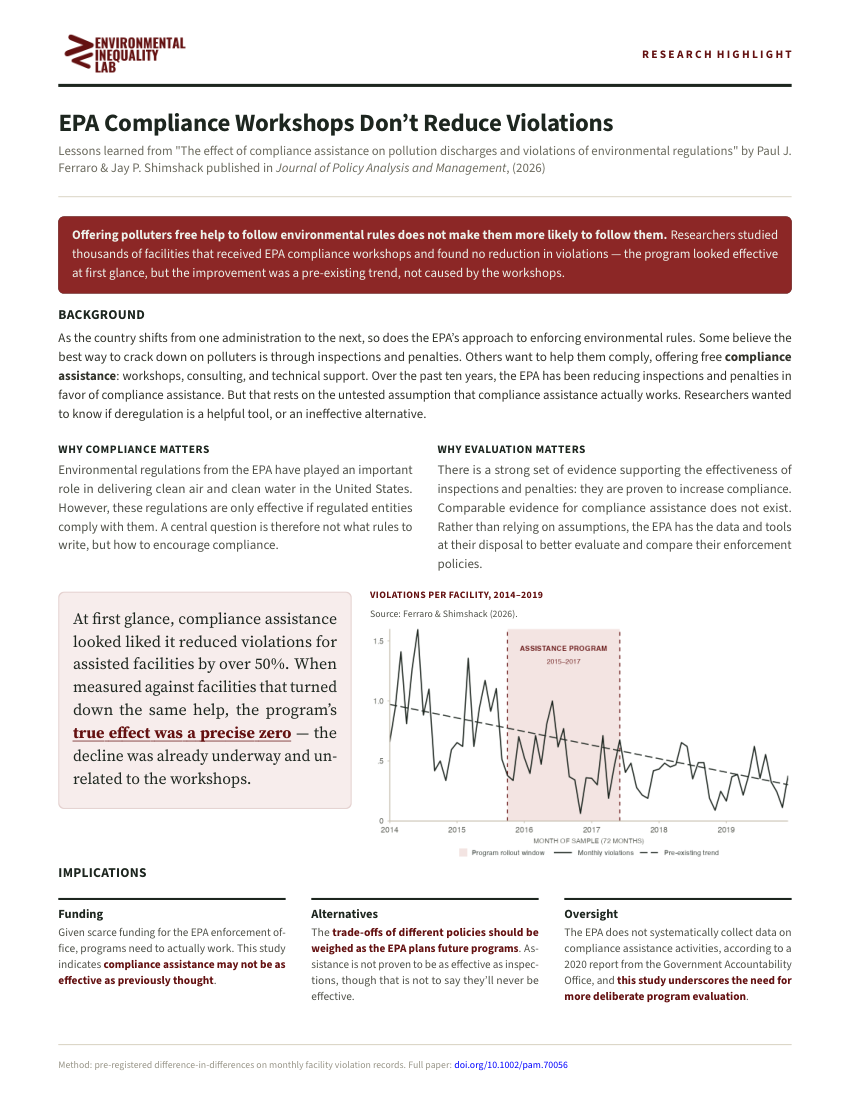
\includegraphics[width=0.85\linewidth]{assets/versions/v1.png}\\[2pt]
      {\footnotesize \textbf{v1}}
    \end{minipage}%
    \begin{minipage}[t]{0.09\textwidth}
      \centering\Large $\rightarrow$
    \end{minipage}%
    \begin{minipage}[t]{0.27\textwidth}
      \centering
      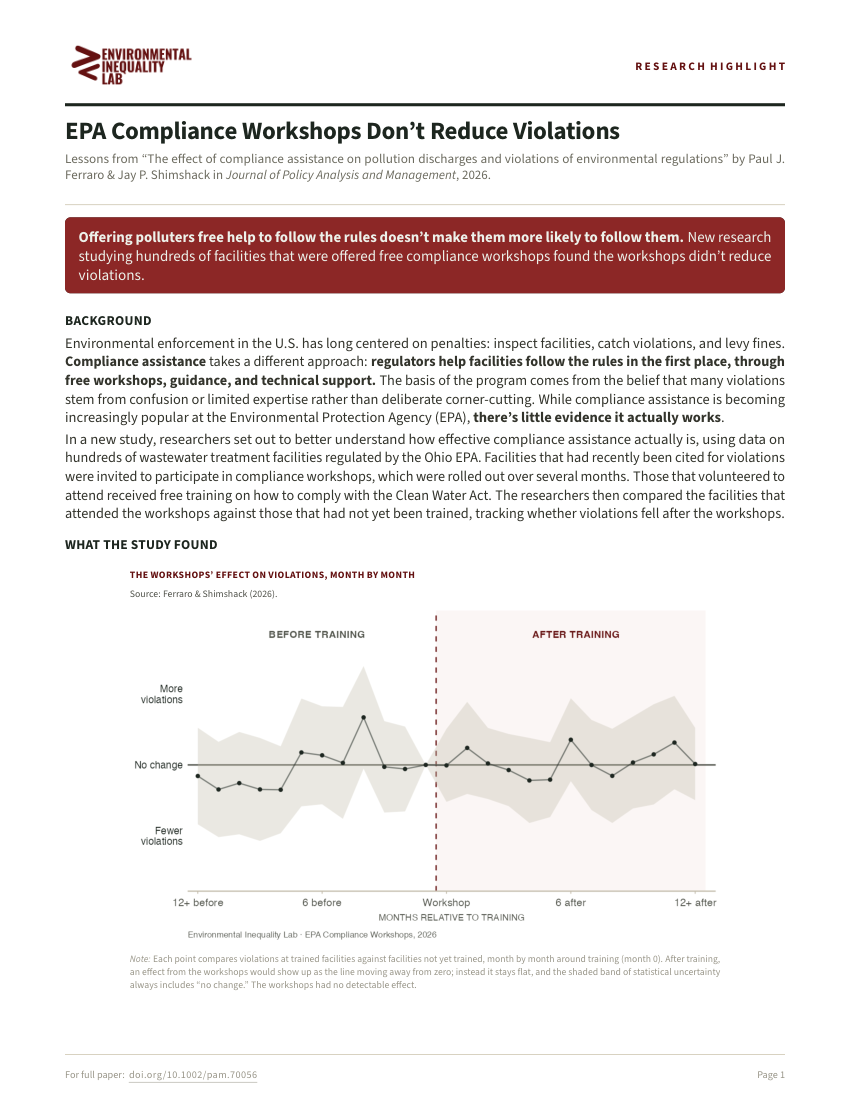
\includegraphics[width=0.85\linewidth]{assets/versions/v4.png}\\[2pt]
      {\footnotesize \textbf{v4}}
    \end{minipage}%
    \begin{minipage}[t]{0.09\textwidth}
      \centering\Large $\rightarrow$
    \end{minipage}%
    \begin{minipage}[t]{0.27\textwidth}
      \centering
      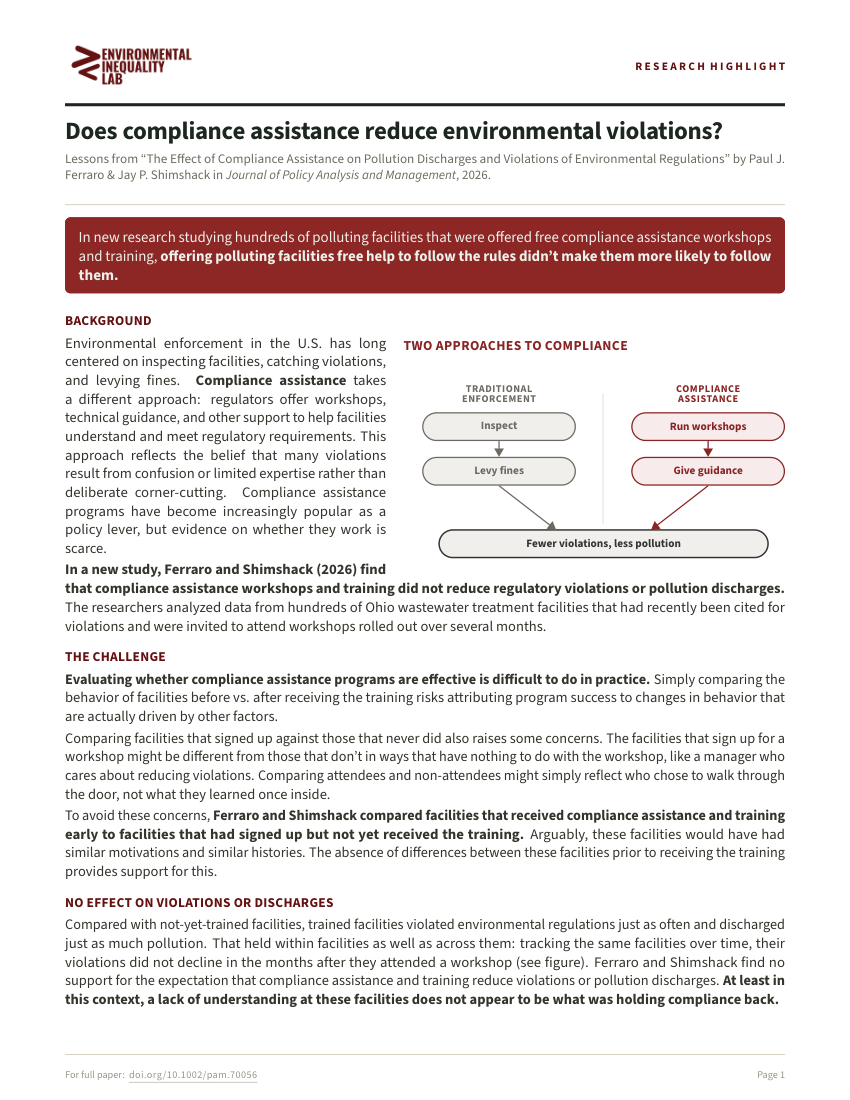
\includegraphics[width=0.85\linewidth]{assets/versions/v10.png}\\[2pt]
      {\footnotesize \textbf{v10}}
    \end{minipage}
  \end{center}
\end{frame}

% ---------------------------------------------------------------------
\begin{frame}{Case Study: EPA Compliance Workshops --- The Output}
  \vfill
  \begin{center}
    \begin{minipage}[t]{0.28\textwidth}
      \centering
      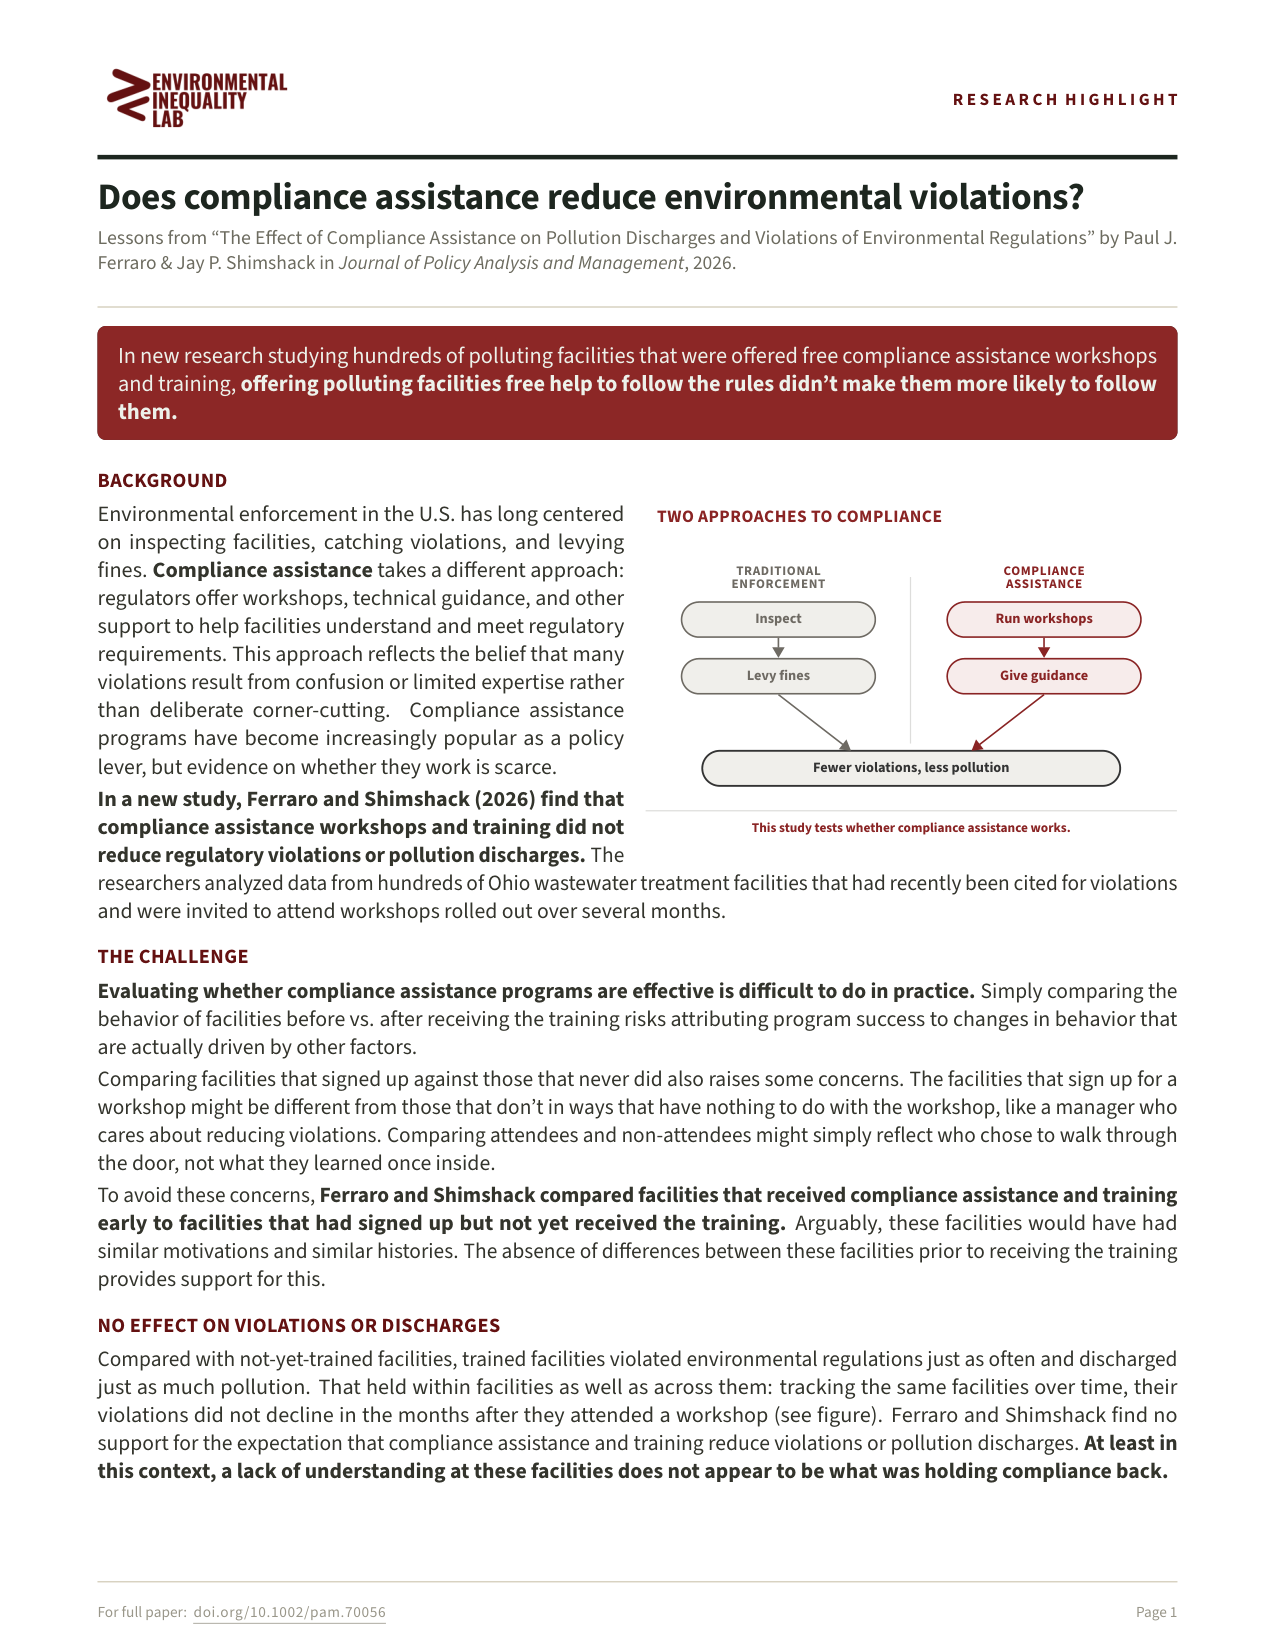
\includegraphics[height=3.4cm]{assets/hl-cover.png}\\[4pt]
      {\footnotesize Research highlight}
    \end{minipage}%
    \hspace{16pt}%
    \begin{minipage}[t]{0.28\textwidth}
      \centering
      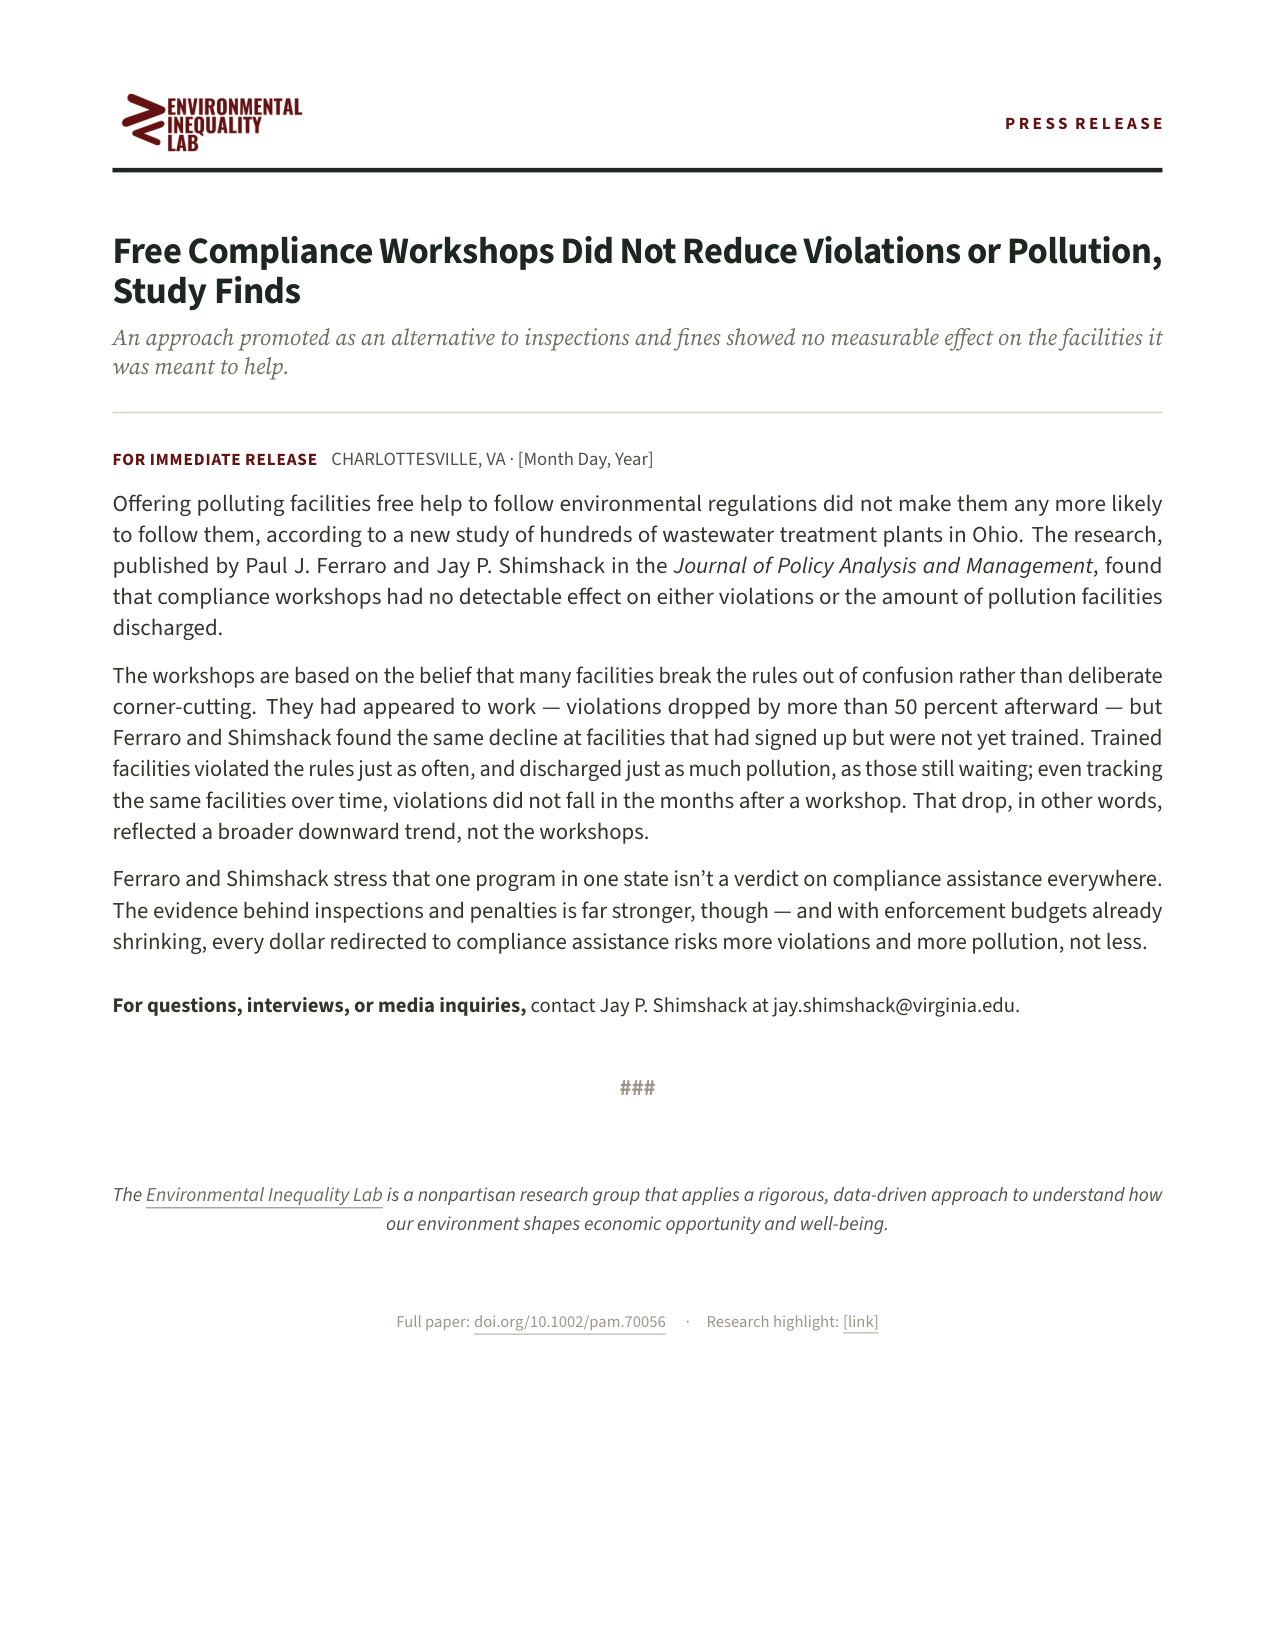
\includegraphics[height=3.4cm]{assets/pr-cover.png}\\[4pt]
      {\footnotesize Press release}
    \end{minipage}%
    \hspace{16pt}%
    \begin{minipage}[t]{0.28\textwidth}
      \centering
      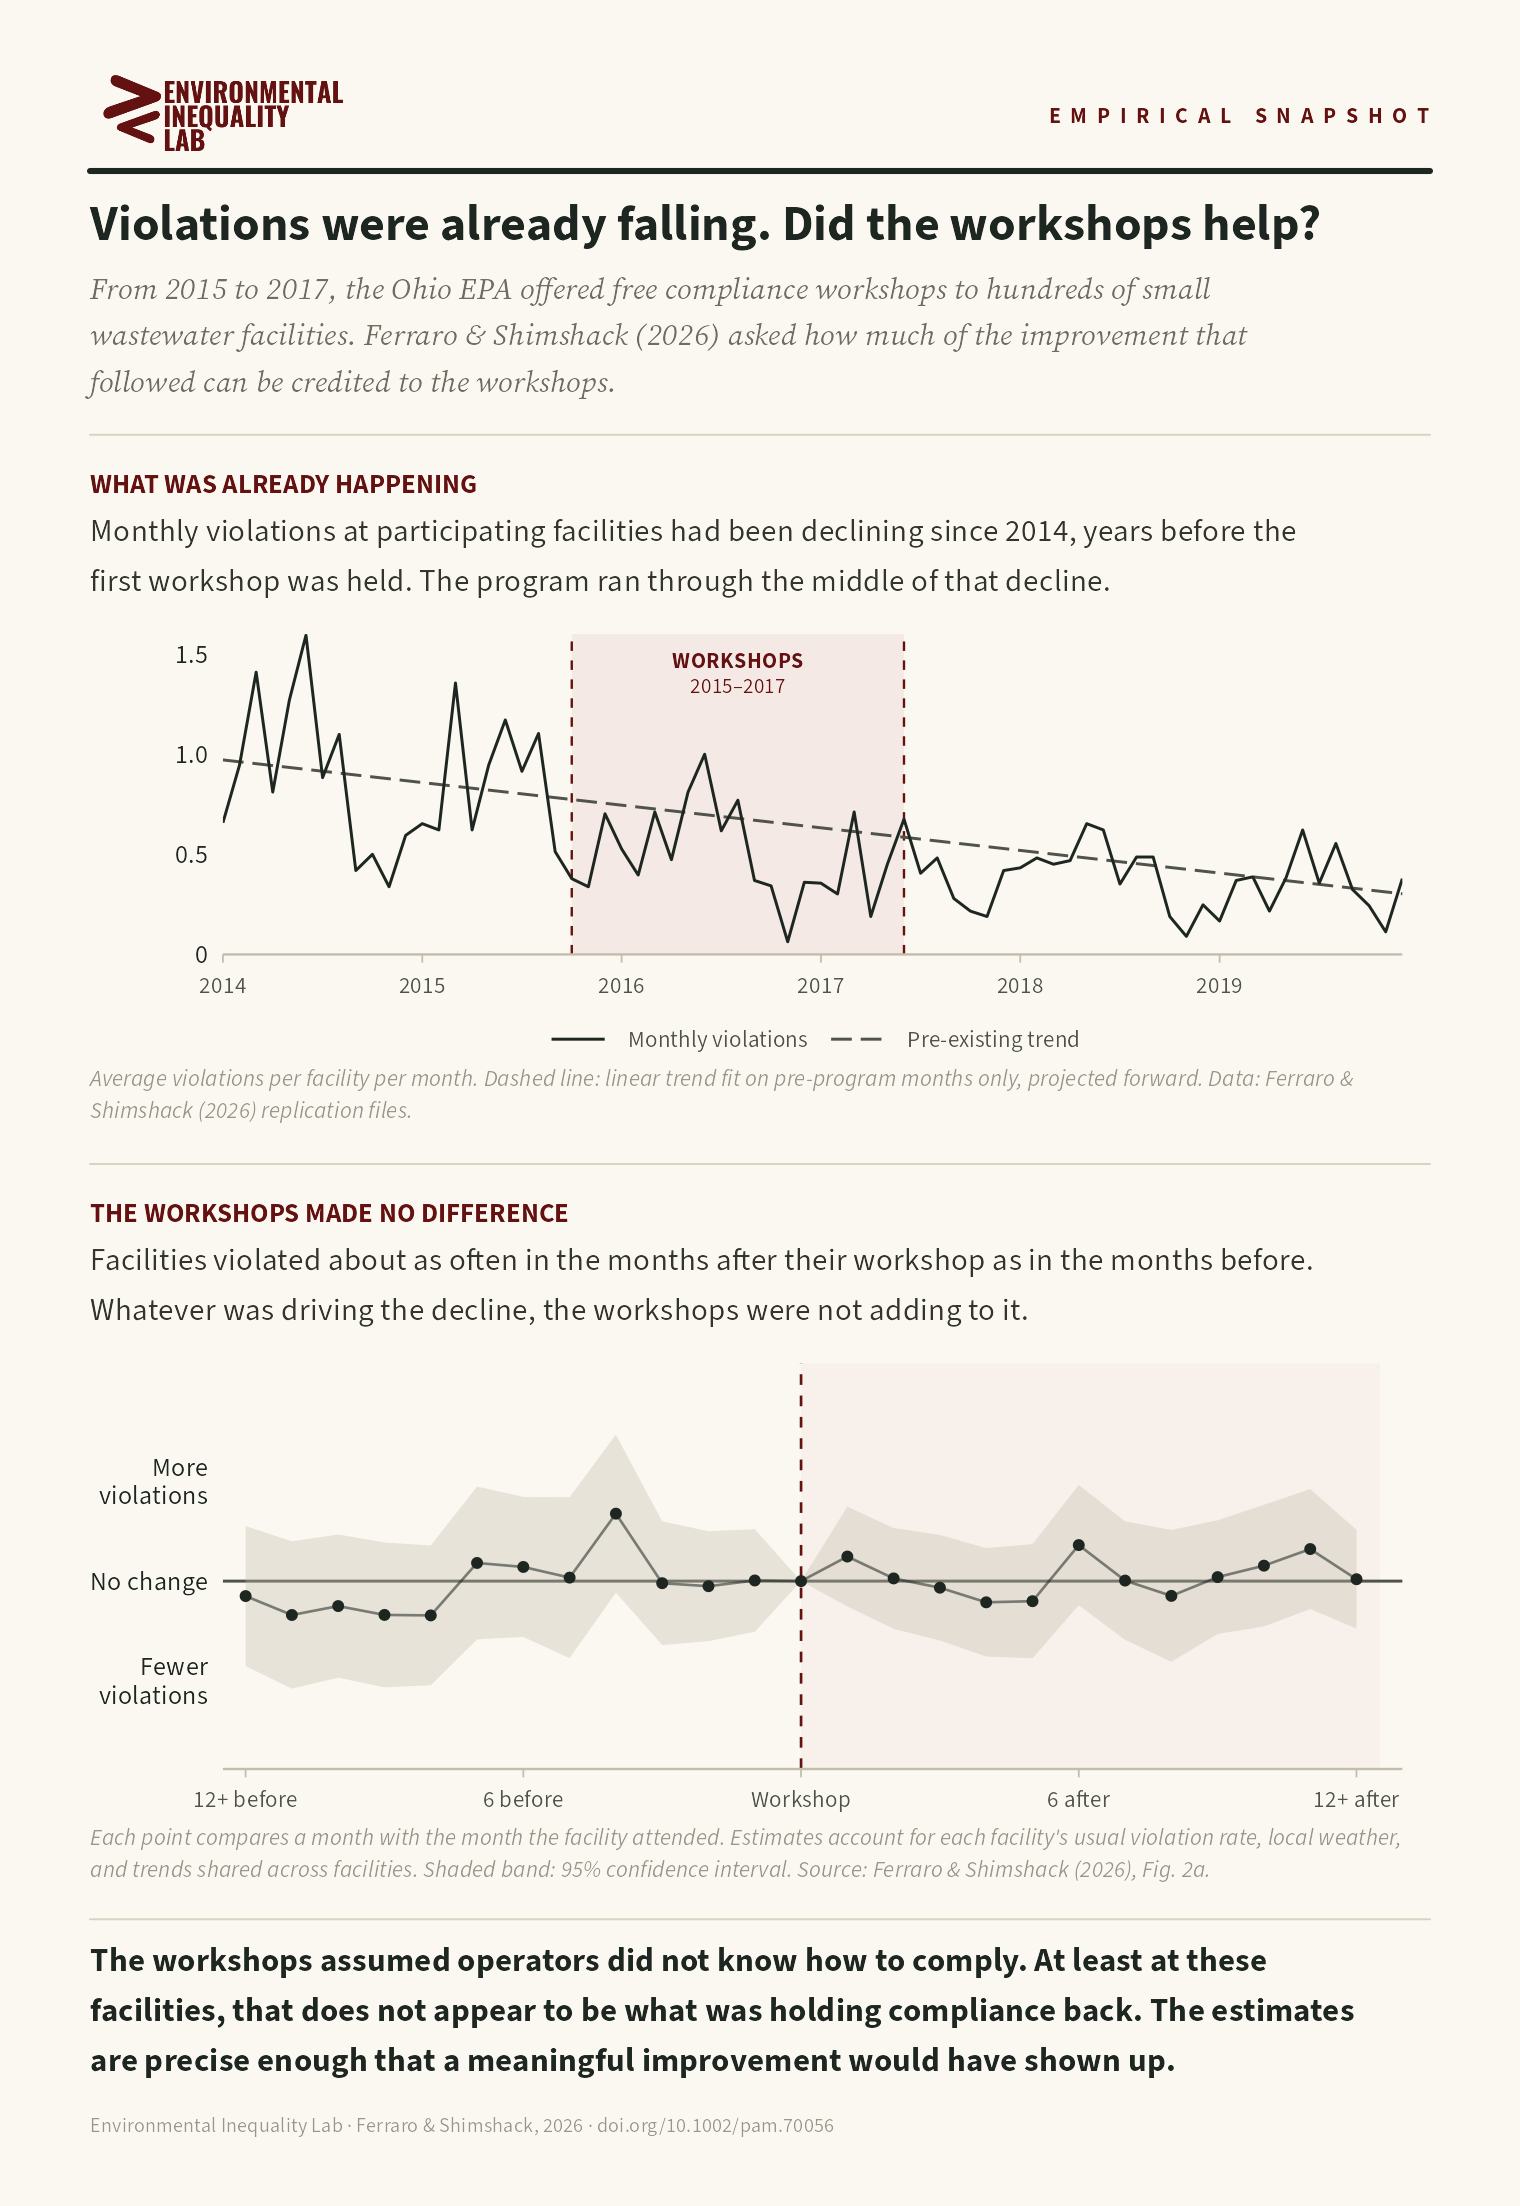
\includegraphics[height=3.4cm]{../../papers/2026-epa-compliance-workshops/empirical-snapshot/figures/option-a-the-reveal.png}\\[4pt]
      {\footnotesize Empirical snapshot}
    \end{minipage}
  \end{center}
  \vfill
  \begin{center}
    \includegraphics[height=1.7cm]{../../papers/2026-epa-compliance-workshops/social/assets/epa-stat-card.png}\hspace{10pt}%
    \includegraphics[height=1.7cm]{../../papers/2026-epa-compliance-workshops/social/assets/epa-chart-card.png}\hspace{10pt}%
    \includegraphics[height=1.7cm]{../../papers/2026-epa-compliance-workshops/social/assets/epa-quote-card.png}\\[4pt]
    {\footnotesize Three social cards}
  \end{center}
  \vfill
\end{frame}

% ---------------------------------------------------------------------
\begin{frame}{Handoff Idea: Rethinking the Website}
  \begin{center}
    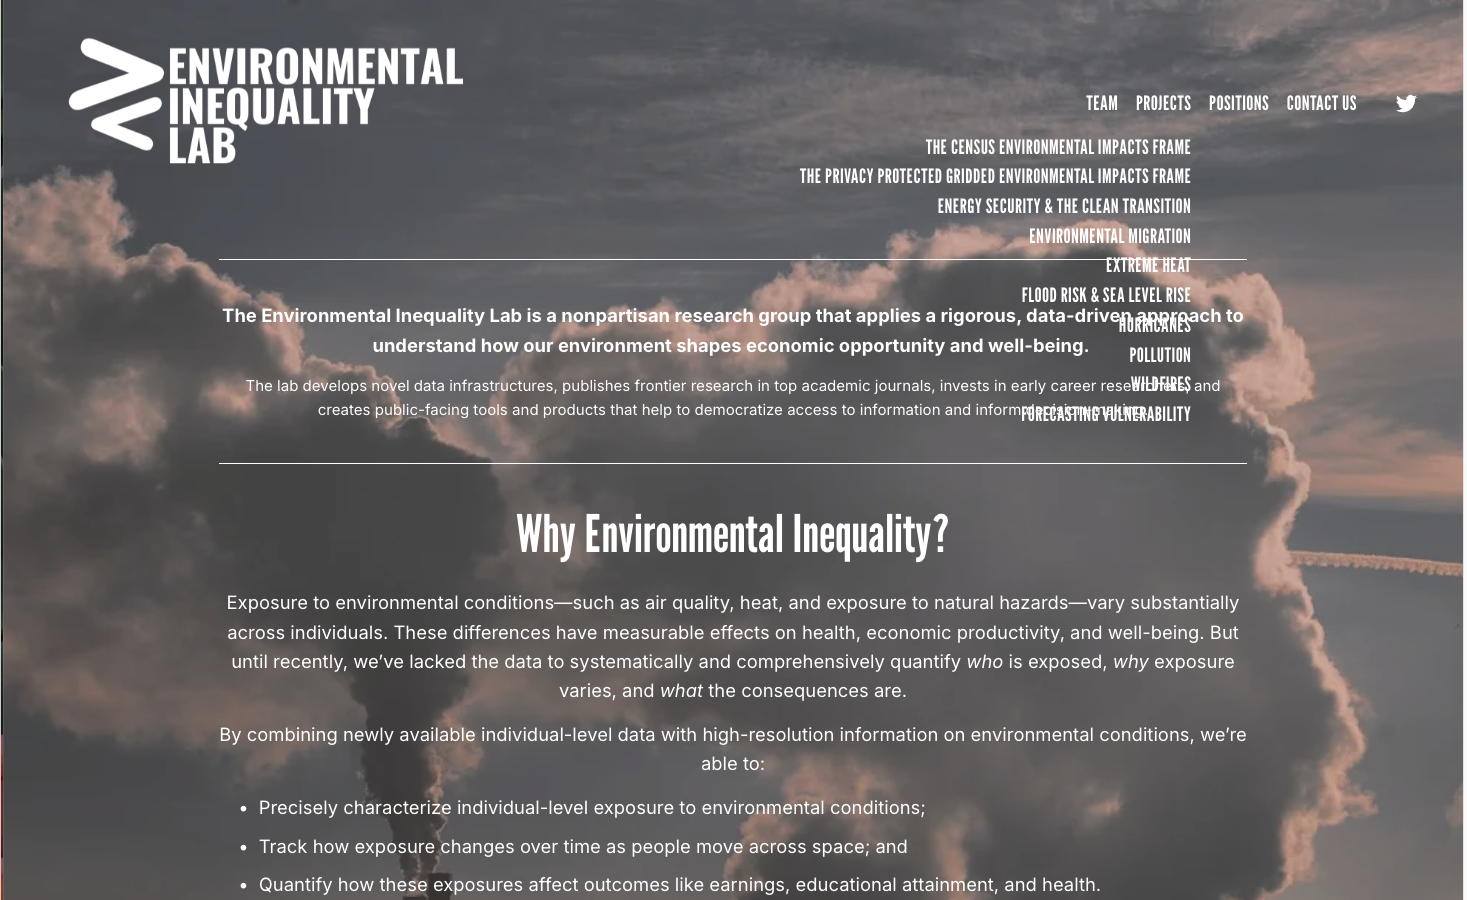
\includegraphics[width=0.56\textwidth]{assets/website-gap.png}
  \end{center}
  \vspace{3pt}
  \begin{center}
    Project pages don't link to any highlight, press release, or social post.\\[6pt]
    \textbf{Proposal:} add them to each project page, plus a site-wide index.
  \end{center}
\end{frame}

% ---------------------------------------------------------------------
\begin{frame}{Handoff Idea: Social Media}
  \begin{center}
    \Large
    Could apply the same idea to social media.\\[14pt]
    \large Missing: account access + a clear mandate\\[10pt]
    \textbf{Open question:} what's social media actually for?
  \end{center}
\end{frame}

% ---------------------------------------------------------------------
\begin{frame}{What I Learned --- Skills \& Workflow}
  \begin{center}
  \Large
  \begin{tabular}{@{}l@{}}
    R \& \TeX{} (figures, graphics, PDFs) \\[10pt]
    Replicability \& version control \\[10pt]
    PI interviews $\rightarrow$ framing (\& press release) \\[10pt]
    Directing AI tools --- prompting, verifying, iterating
  \end{tabular}
  \end{center}
\end{frame}

% ---------------------------------------------------------------------
\begin{frame}{What I Learned --- Judgment \& Research Exposure}
  \begin{center}
  \Large
  \begin{tabular}{@{}l@{}}
    Accessible language for research \& findings \\[10pt]
    Engaging writing vs.\ honest caveats \\[10pt]
    ``What's the point of this?''
  \end{tabular}
  \end{center}
\end{frame}

% ---------------------------------------------------------------------
\begin{frame}{Personal Takeaways}
  \vfill
  \begin{center}
    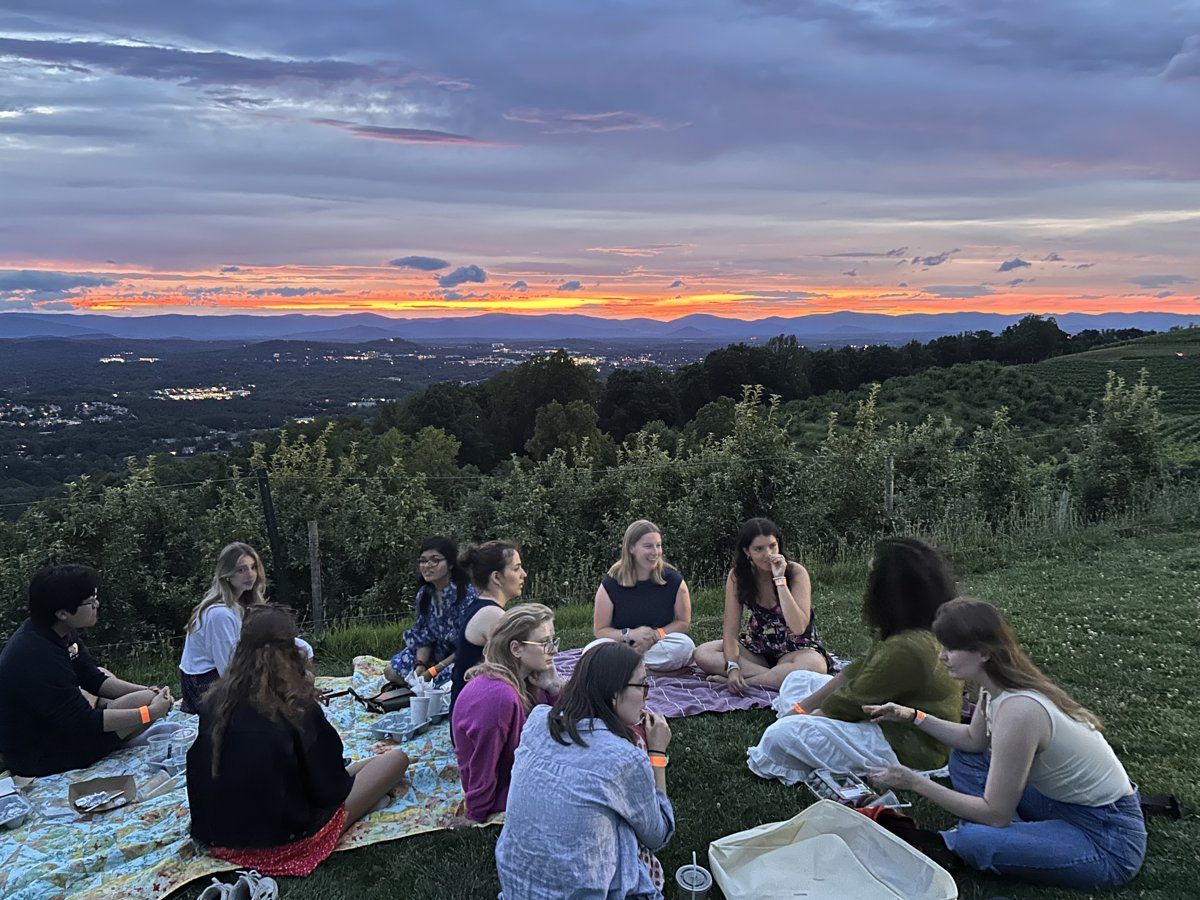
\includegraphics[height=2.6cm]{assets/personal/picnic.jpg}\hspace{8pt}%
    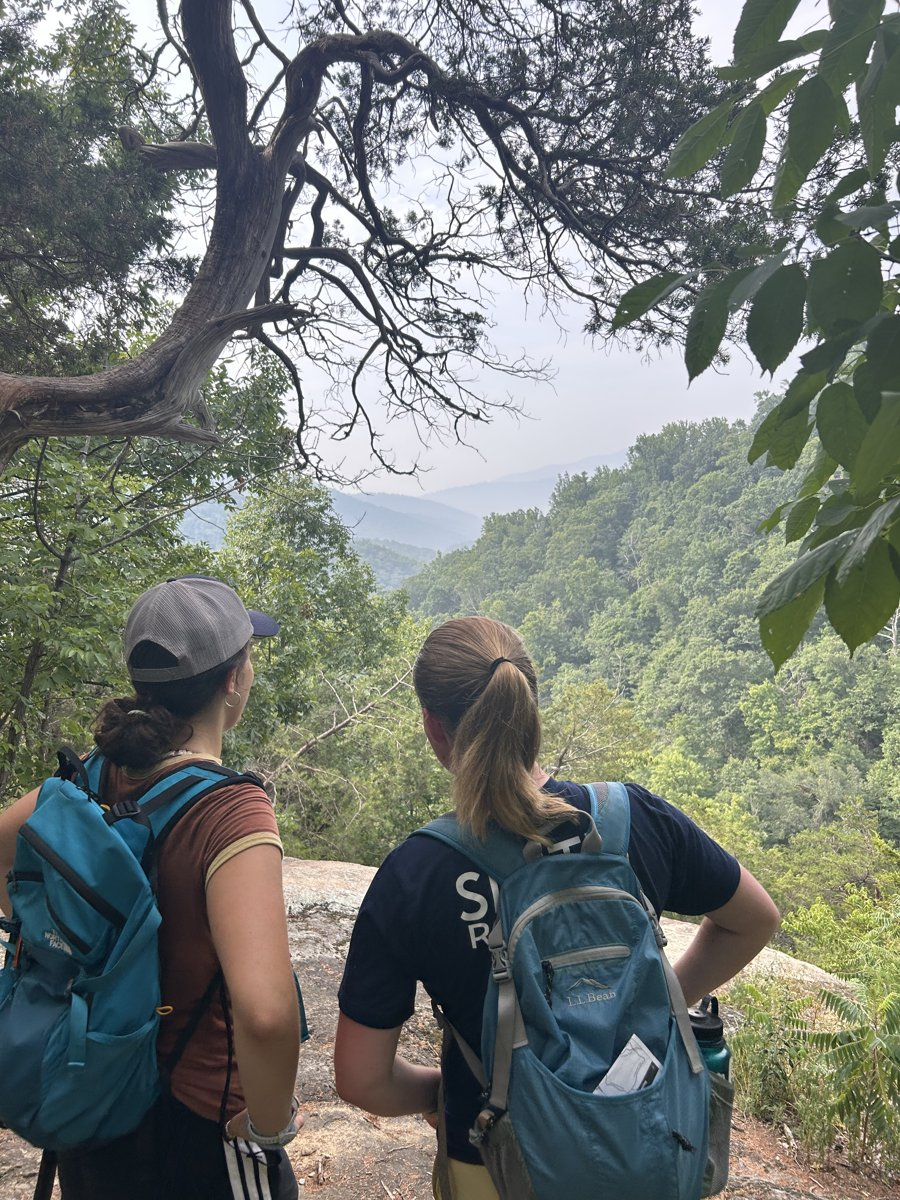
\includegraphics[height=2.6cm]{assets/personal/hike.jpg}\hspace{8pt}%
    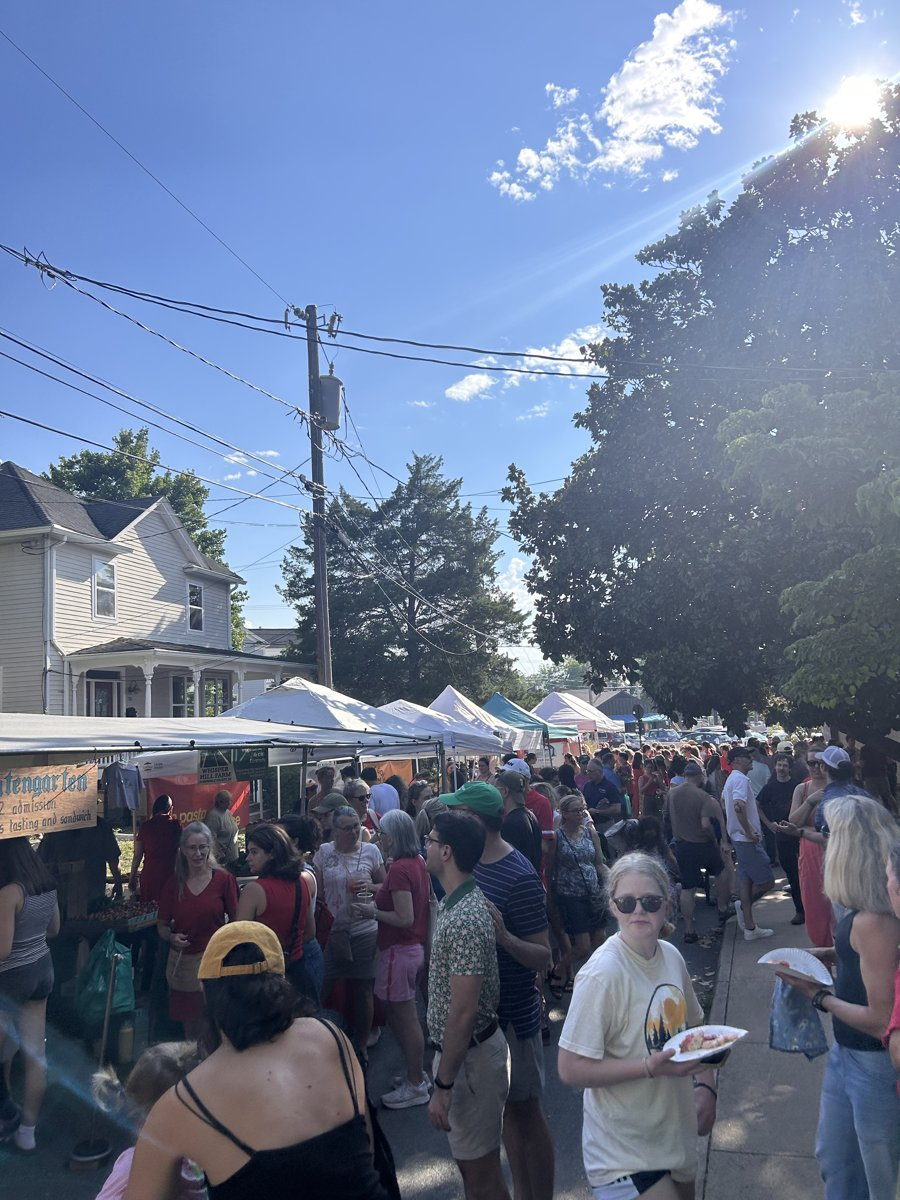
\includegraphics[height=2.6cm]{assets/personal/festival.jpg}\hspace{8pt}%
    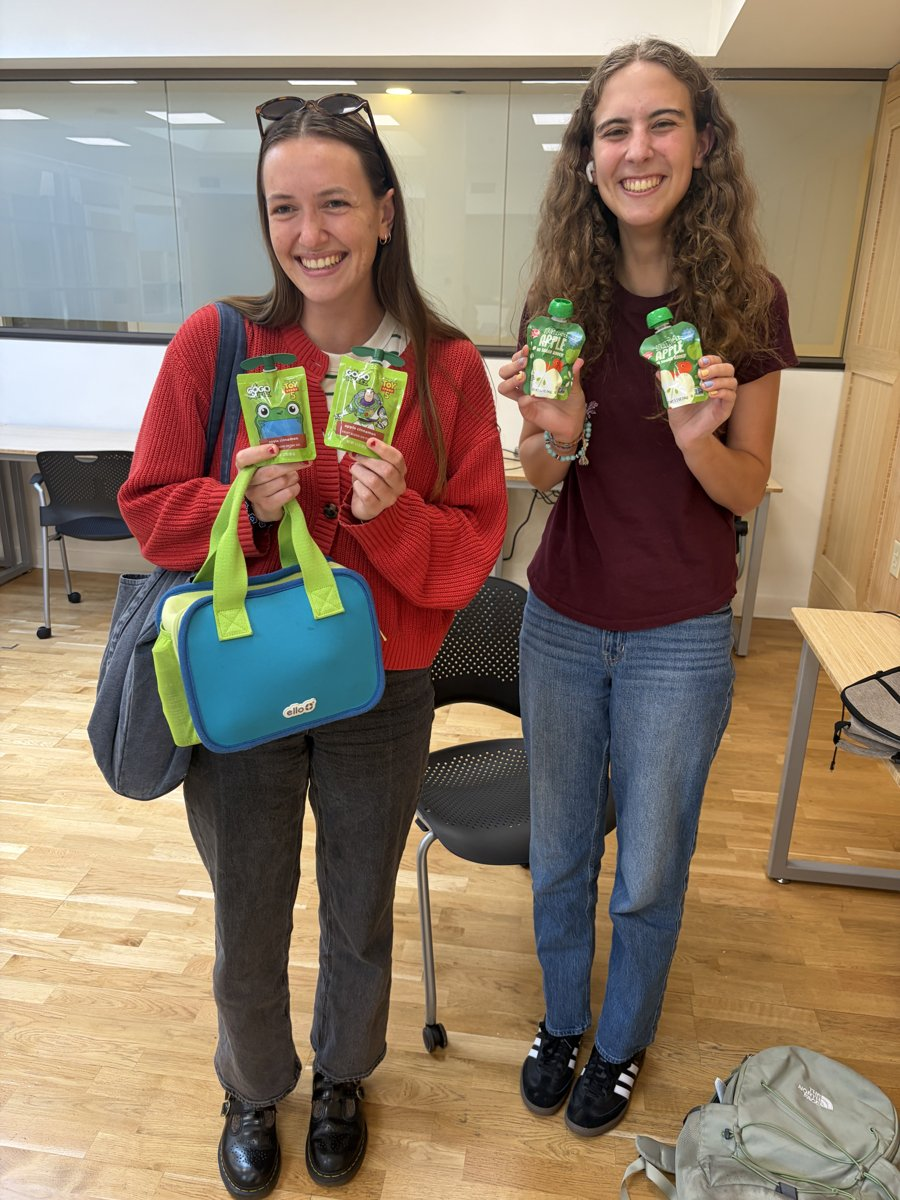
\includegraphics[height=2.6cm]{assets/personal/office.jpg}
  \end{center}

  \vspace{8pt}
  \begin{center}
    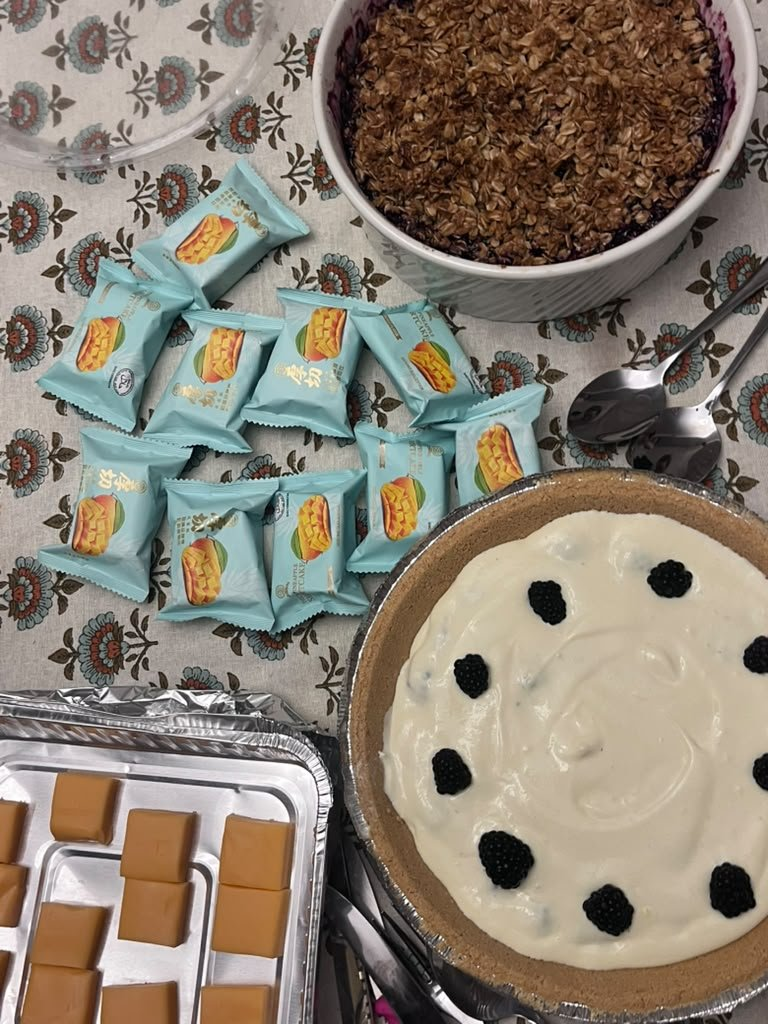
\includegraphics[height=2.6cm]{assets/personal/desserts.jpg}\hspace{8pt}%
    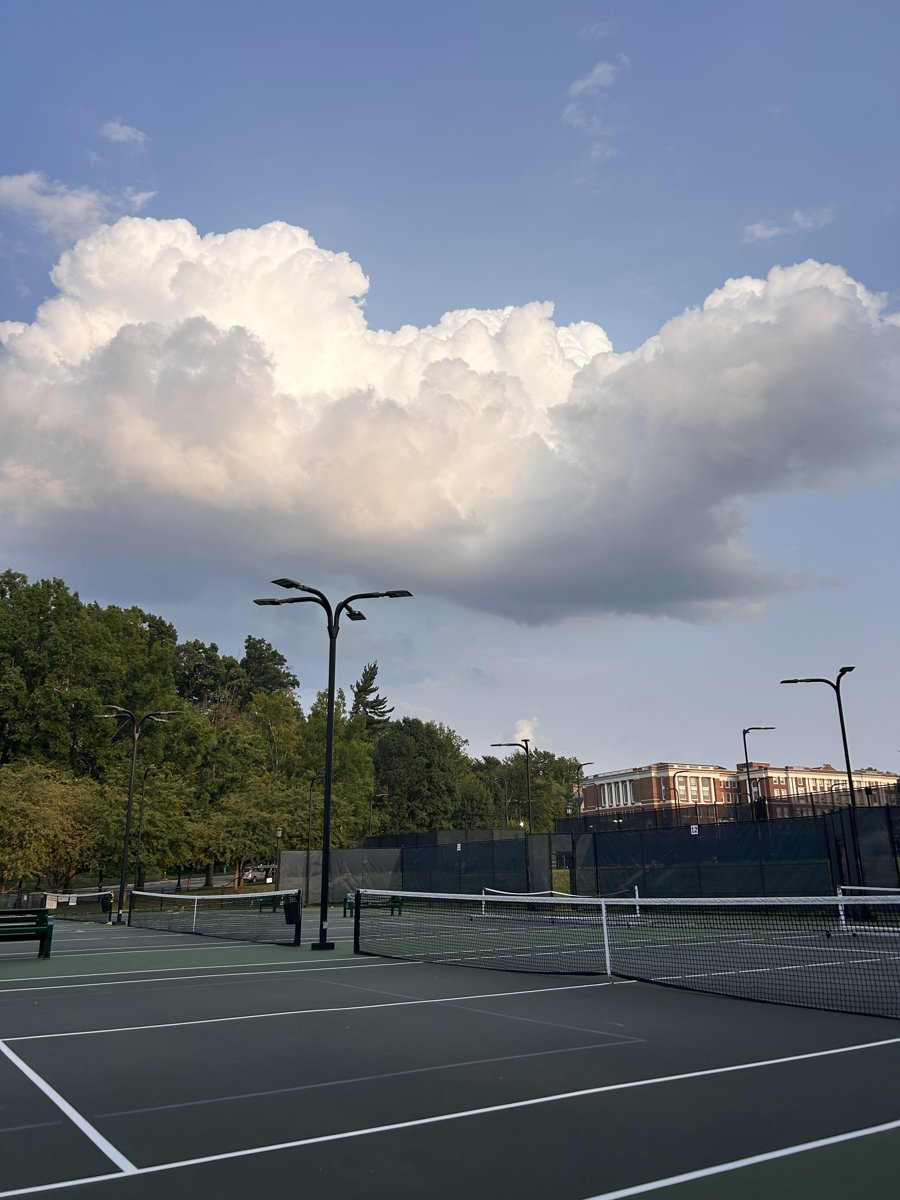
\includegraphics[height=2.6cm]{assets/personal/storm.jpg}\hspace{8pt}%
    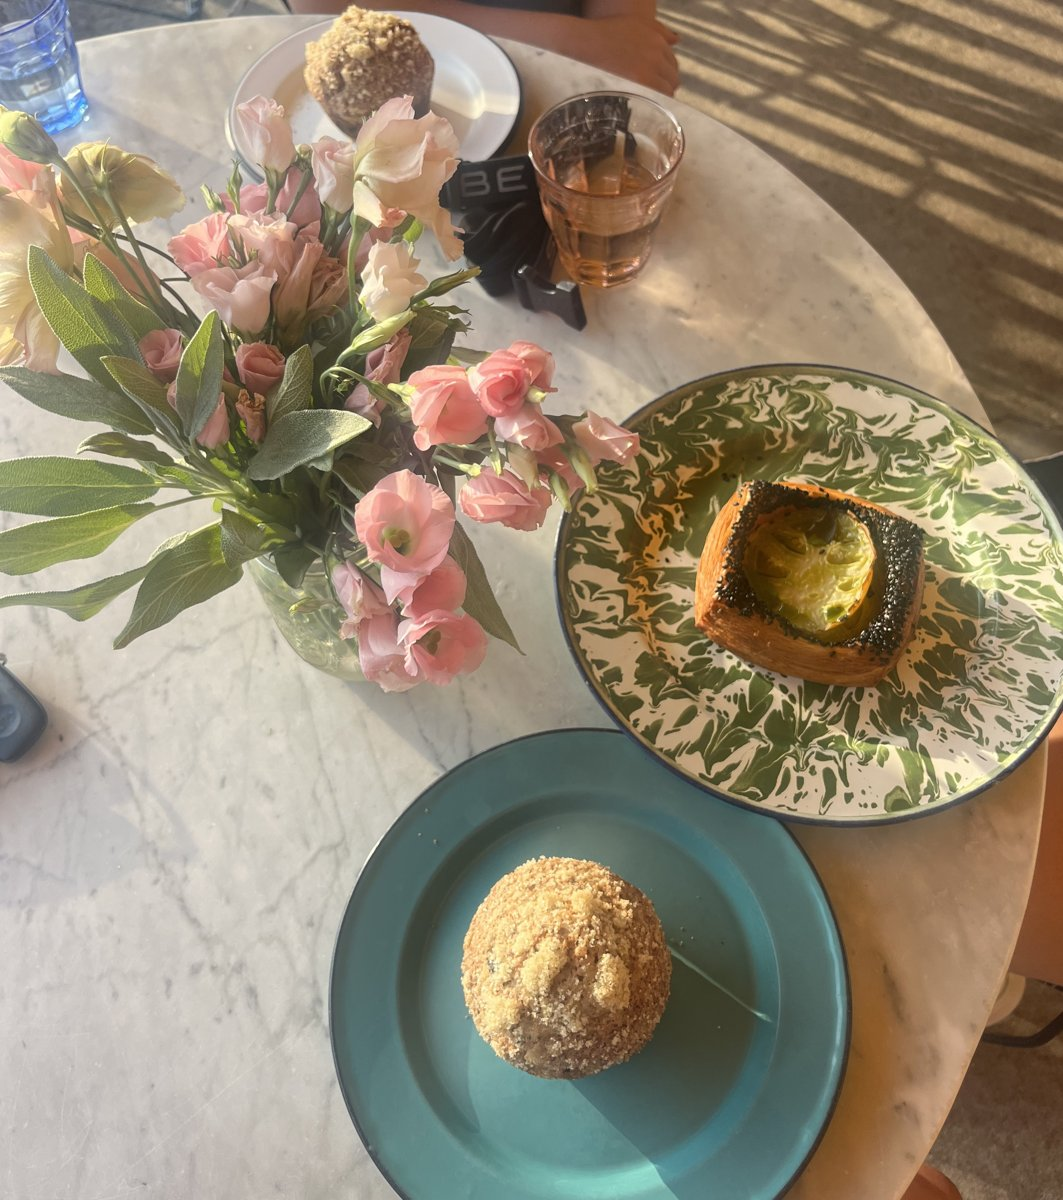
\includegraphics[height=2.6cm]{assets/personal/brunch.jpg}
  \end{center}
  \vfill
  \begin{center}
    The work was especially fulfilling surrounded by smart, hard-working, supportive colleagues.
  \end{center}
  \vfill
\end{frame}

% ---------------------------------------------------------------------
\begin{frame}[standout]
  Thank you --- Questions?
\end{frame}

\end{document}
